\documentclass[12pt]{article}
\usepackage{notes-common}
\usepackage{graphicx}
\geometry{margin=0.35in}
\AtBeginDocument{\fontsize{14}{17}\selectfont}

% Complete / filled-in reference version of wire-force-levitation-notes.tex.
\newcommand{\eqline}[2][-0.5mm]{%
  \par\vspace{1mm}\noindent #2\par\vspace{#1}%
  \noindent\textcolor{rulehue}{\rule{\linewidth}{0.5pt}}\par\vspace{4mm}%
}
\newcommand{\ANS}[1]{\textcolor{accent}{#1}}

\begin{document}

\noteshead{Magnetic Force on a Current-Carrying Wire \textcolor{accent}{(completed)}}{}

\goal{
\begin{itemize}[itemsep=5pt,parsep=2pt,topsep=2pt]
\item See where the force on a current-carrying wire, $F=IlB\sin\alpha$,
comes from --- it's just $q\vec v\times\vec B$ summed over every moving
charge in the wire.
\item Use the right-hand rule both ways: given $I$ and $\vec B$, find
$\vec F$; and given the $\vec F$ you need, find the current direction
that produces it.
\item Work a full numerical example end to end: find the current that
lets a wire ``float'' against gravity in a magnetic field (Example
29.13).
\end{itemize}}

%============================================================
\nsec{Where the force on a wire comes from}

A current is moving charge. A short segment of wire, length $\Delta x$,
carrying charge $\Delta q$ with drift velocity $\vec v_{\text d}$, feels
the same magnetic force as any moving charge: $F=\Delta q\,v_{\text
d}B$. The charge crosses the segment in a time $\Delta t=\Delta
x/v_{\text d}$, so $\Delta q = \ANS{I\,\Delta t}$ (in terms of $I$ and
$\Delta t$). Substituting:

\[
F = \Delta q\, v_{\text d} B = \ANS{\dfrac{\Delta q}{\Delta t}(v_{\text
d}\Delta t)B = I\,\Delta x\, B}
\]

Adding up every such segment over the full length $l$ of wire (when
the wire is perpendicular to $\vec B$) gives $F=IlB$. More generally,
for a wire at angle $\alpha$ to the field:

\result[1.8cm]{$\vec F_{\text{wire}} = \ANS{I\vec l\times\vec B =
(IlB\sin\alpha,\ \text{direction by right-hand rule})}$}

\checkpoint{The box above should look just like the moving-charge
force law $\vec F = q\vec v\times\vec B$, with two substitutions. What
plays the role of $q$, and what plays the role of $\vec v$?}

{\small\color{accent} The combination $I\vec l$ plays the role of
$q\vec v$ --- current times length stands in for ``how much charge is
moving, how fast,'' just as it did when this same force law was first
built up from the individual charge carriers.}

\textbf{NOTE} --- Right-hand rule for a current-carrying wire: point
your right \ANS{thumb} in the direction of the current (parallel to
$\vec l$), your \ANS{index finger} in the direction of $\vec B$. Your
\ANS{middle finger} then points along $\vec F$.

%============================================================
\nsec{Worked example: magnetic levitation (Example 29.13)}

\textit{A uniform field $B=0.10$ T is horizontal, parallel to the
floor. A straight segment of 1.0-mm-diameter copper wire, also
parallel to the floor, is perpendicular to the field. What current
through the wire, and in which direction, will allow the wire to
``float'' in the magnetic field?}

\begin{center}
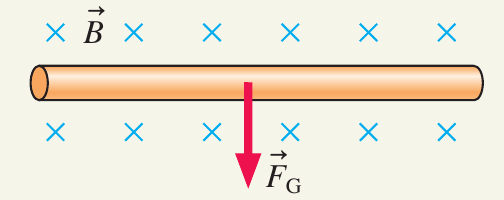
\includegraphics[width=0.55\linewidth]{figures/knight-fig29-44.png}
\end{center}
\figtask{Label $\vec B$'s direction, and sketch in the current
direction and $\vec F_B$ once you've worked out which way they go.}

\textbf{MODEL.} The wire floats if the magnetic force on it points
\ANS{upward} and has magnitude \ANS{$mg$}, exactly balancing the
downward gravitational force.

\textbf{SOLVE --- set the forces equal.} With the wire perpendicular
to $\vec B$:

\[
F = IlB = \ANS{mg}
\]

The weight comes from the copper's density $\rho=8920\text{ kg/m}^3$
and the wire's volume. Write the mass as $m=\rho V$, with $V$ the
volume of a cylinder of radius $r$ and length $l$:

\[
IlB = \ANS{\rho(\pi r^2 l)g}
\]

\checkpoint{One factor appears on both sides of that equation and
cancels. Which one --- and why should the current needed to float the
wire \emph{not} depend on how long the wire is?}

{\small\color{accent} The length $l$ cancels. A longer wire weighs
proportionally more ($mg\propto l$), but it also feels proportionally
more magnetic force for the same current ($F\propto l$) --- the two
effects grow together, so the current that balances them is the same
no matter how long the segment is.}

Solve for the current:

\result[1.8cm]{$I = \ANS{\dfrac{\rho\pi r^2 g}{B}}$}

Plug in $r=0.00050$ m, $g=9.80\text{ m/s}^2$, and the given $B$ and
$\rho$:

\eqline[0.2cm]{$I = \ANS{\dfrac{(8920)\pi(0.00050)^2(9.80)}{0.10} =
0.69\text{ A}}$}

\textbf{Direction.} With $\vec B$ pointing into the page (as drawn),
the right-hand rule says the current must flow \ANS{left to right} to
make $\vec F_B$ point \ANS{up}.

\checkpoint{The book notes this idea is only useful once you can get
current into and out of the floating segment. If the lead-in wires run
straight down to the segment (parallel to $\vec B$), why do \emph{they}
feel no force while the segment does?}

{\small\color{accent} $\vec F=I\vec l\times\vec B$ vanishes whenever
$\vec l$ and $\vec B$ are parallel (or antiparallel) --- $\sin\alpha=0$
there. The lead-in wires run along $\vec B$'s direction, so they feel
no magnetic force at all; only the horizontal segment, which is
perpendicular to $\vec B$, does.}

\end{document}
